\subsection{Newton-Raphson and Secant Methods}

\frame{
\frametitle{Slope Methods for Finding Roots}
\begin{block}{}
If $f (x)$, $f'(x)$, and $f''(x)$ are continuous near a root $p$, then this extra information regarding the nature of $f (x)$ can be used to develop algorithms that will produce sequences $\{ p_k \}$ that converge faster to $p$ than either the bisection or false position method.
\end{block}

{\Large The Newton-Raphson (or simply Newton’s) method is one of the most useful and best known algorithms that relies on the continuity of $f'(x)$ and $f''(x)$. }
}

\frame{
Assume that the initial approximation $p_0$ is near the root p.  \\
\begin{itemize}
\item Then the graph of $y = f (x)$ intersects the x-axis at the point $(p, 0)$, and the point $(p_0, f(p_0))$ lies on the curve near the point $(p, 0)$. 
\item Define $p_1$ to be the point of intersection of the x-axis and the line tangent to the curve at the point $(p_0, f(p_0))$.
\end{itemize}
\begin{figure}
\begin{center}
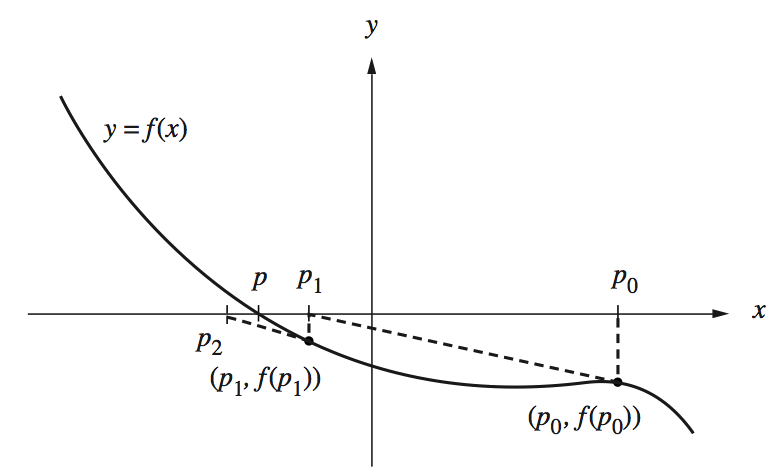
\includegraphics[width=60mm]{chap-1/fig_2-13.png}
\end{center}
\end{figure}
\begin{block}{}
It is shown that $p_1$ will be closer to $p$ than $p_0$ in this case.
\end{block}
}


\frame{
An equation relating $p_1$ and $p_0$ can be found if we write down two versions for the slope of the tangent line $L$:
\begin{equation*}
m = \frac{0 - f(p_0)}{p_1-p_0} 
\end{equation*}
which is the slope of the line through $(p_1, 0)$ and $(p_0, f(p_0))$,  and
\begin{equation*}
m =  f'(p_0) 
\end{equation*}
which is the slope at the point $(p_0, f(p_0))$. \\
\begin{center}
$\Downarrow $
\end{center}
\begin{equation*}
p_1 =  p_0 - \frac{f(p_0)}{f'(p_0)} 
\end{equation*}
\begin{block}{}
This process can be repeated to obtain a sequence $\{ p_k \}$ that converges to $p$.
\end{block}
}

\frame{
\begin{block}{Theorem (Newton-Raphson Theorem)}
Assume that $f \in C^2[a, b]$ and there exists a number $p \in [a, b]$, where $f(p) = 0$. 
If $f'(p) \neq 0$, then there exists a $\delta > 0$ such that the sequence $\{p_k\}^{\infty}_{k=0}$ defined by the iteration
\begin{equation*}
p_k = g(p_{k-1}) =  p_{k-1} - \frac{ f(p_{k-1}) }{ f'(p_{k-1}) }  \ \ \ for \ \ \ k=1,2,\ldots
\end{equation*}
will converge to $p$ for any initial approximation $p_0 \in [p - \delta, p + \delta]$.
\end{block}
\begin{block}{Remark}
The function $g(x)$ defined by the formula
\begin{equation*}
 g(x) = x - \frac{ f(x) }{ f'(x) } 
\end{equation*}
is called the {\Large Newton-Raphson iteration function}.
\end{block}
}

\frame{
\frametitle{Proof of Theorem}
The Taylor polynomial of degree $n = 1$ and its remainder term:
\begin{equation*}
 f(x) = f(p_0)  + f'(p_0) (x - p_0) + \frac{ f''(c) (p-P_0)^2 }{ 2! } 
\end{equation*}
where $c$ lies somewhere between $p_0$ and $x$.
\begin{center}
$\Downarrow $
\end{center}
Substituting $x = p$ into the equation  and using the fact that $f (p) = 0$ produces
\begin{equation*}
 0 = f(p_0)  + f'(p_0) (x - p_0) + \frac{ f''(c) (p-P_0)^2 }{ 2! } 
\end{equation*}
}

\frame{
\frametitle{Proof of Theorem  (continued)}
If $p_0$ is close enough to $p$, the last term on the right side of above function\footnote{ Taylor polynomial} will be small compared to the sum of the first two terms.
\begin{center}
$\Downarrow $
\end{center}
Hence it can be neglected and we can use the approximation
\begin{equation*}
 0 \approx f(p_0)  + f'(p_0) (x - p_0)  
\end{equation*}
\begin{center}
$\Downarrow $
\end{center}
Solving for $p$ in the equation, we get $p \approx p_0 - f (p_0) \/ f'(p0)$.
\begin{center}
$\Downarrow $
\end{center}
This is used to define the next approximation p1 to the root
\begin{equation*}
p_1 \approx p_0  - \frac{f(p_0)}{ f' (p_0)}
\end{equation*}
}

\frame{
\frametitle{Proof of Theorem (continued)}
\begin{center}
$\Downarrow $
\end{center}
When $p_{k-1}$ is used in place of $p_0$ in equation, the general rule is established.
\begin{center}
$\Downarrow $
\end{center}
However, to fully comprehend what is happening, we need to consider the fixed-point iteration function and apply Theorem 1.2 in our situation.
The key is in the analysis of $g'(x)$:
\begin{equation*}
g'(x)   = 1 - \frac{f'(x)f'(x) - f(x)f''(x)}{(f'(x))^2 } =   \frac{f(x)f''(x)}{(f'(x))^2 }
\end{equation*}
}

\frame{
\frametitle{Proof of Theorem (continued)}
Since $g'(p) = 0$ and $g'(x)$ is continuous,  
it is possible to find a $\delta > 0$ so that the hypothesis $| g'(x) | < 1$ is satisfied on $( p - \delta, p + \delta )$.
\begin{center}
$\Downarrow $
\end{center}
Therefore, a sufficient condition for $p_0$ to initialize a convergent sequence $\{ p_k \}^{\infty}_{k=0}$, which converges to a root of $f (x) = 0$, is that $p_0 \in (p - \delta, p + \delta)$ and that $\delta$ be chosen so that
\begin{equation*}
 \frac{| f(x)f''(x)| }{| (f'(x))|^2 } < 1 \ \ \ for \ \ all \ \ x \in  (p - \delta, p + \delta)
\end{equation*}
}

\frame{
\begin{block}{Corollary  (Newton’s Iteration for Finding Square Roots).}
Assume that $A > 0$ is a real number and let $p_0 > 0$ be an initial approximation to $\sqrt{A}$.
Define the sequence $\{ p_k \}^{\infty}_{k =0}$ using the recursive rule
\begin{equation*}
p_k = \frac{p_{k-1}+\frac{A}{p_{k-1}}}{2}
\end{equation*}
for $k =  1, 2, \ldots$
Then the sequence $\{ p_k \}^{\infty}_{k =0}$ converges to $\sqrt{A}$; that is, $\lim_{n \rightarrow \infty} p_k = \sqrt{A}$.
\end{block}
}

\frame{
\frametitle{Proof of Corollary (Newton’s Iteration for Finding Square Roots).}
Start with the function $f (x) = x^2 - A$, and notice that the roots of the equation $x^2 - A = 0$ are $\pm \sqrt{A}$.
\begin{center}
$\Downarrow $
\end{center}
write down the {\Large Newton-Raphson iteration formula}
\begin{equation*}
g(x) = x - \frac{f(x)}{f'(x)} = x - \frac{x^2 - A}{2x}
\end{equation*}
\begin{center}
$\Downarrow $
\end{center}
This formula can be simplified to obtain
\begin{equation*}
g(x) = x - \frac{x+\frac{A}{x}}{2} 
\end{equation*}
}

\frame{
\frametitle{Division-by-Zero Error}
\begin{itemize}
\item One obvious pitfall of the Newton-Raphson method is the possibility of division by zero in the formula, which would occur if $f'(p_{k-1}) = 0$.
\item It is quite possible that $f (p_{k-1})$ is sufficiently close to zero and that $p_{k-1}$ is an acceptable approximation to the root. 
\end{itemize}
\begin{block}{}
We now investigate this situation and will uncover an interesting fact, that is, how fast the iteration converges.
\end{block}
}

\frame{
\begin{block}{Definition.}
Assume that $f (x)$ and its derivatives $f'(x), \ldots, f^{(M)}(x)$ are defined and continuous on an interval about $x = p$. 
We say that $f (x) = 0$ has a {\Large root of order} $M$ at x = p if and only if
\begin{center}
$f(p) = 0$, $f'(p)=0$, $\ldots$, $f^{(M-1)}(p)=0$, and $f^{(M)}(p) \ne 0$
\end{center}
\end{block}
A root of order $M = 1$ is often called a {\Large simple root}, and if $M > 1$, it is called a {\Large multiple root}. 
A root of order $M = 2$ is sometimes called a {\Large double root}, and so on.
}

\frame{
\begin{block}{Lemma(引理).}
If the equation $f (x) = 0$ has a root of order $M$ at $x = p$, then there exists a continuous function $h(x)$ so that $f (x)$ can be expressed as the product
\begin{equation*}
f(x) = (x -p)^M h(x), \ \ \ where \ \ h(p) \ne 0
\end{equation*}
\end{block}
Proof :\\
By the Taylor formula, we can expand $f(x)$ about $x=p$ to get
\begin{equation*}
f(x) = (x-p)^M\frac{f^{(M)}(c(x))}{M!}
\end{equation*}
where $c(x)$ is between $p$ and x.
$h(x)$ is continuous on an interval about $x =p$, and 
\begin{equation*}
h(p) = \lim_{x \rightarrow \infty} \frac{f^{(M)}(c(x))}{M!} = \frac{f^{(M)}(p)}{M!} \ne 0
\end{equation*}
}

\frame{
\frametitle{Speed of Convergence}
\begin{itemize}
\item If $p$ is a simple root of $f (x) = 0$, {\Large Newton’s method} will converge rapidly, and the number of accurate decimal places (roughly) doubles with each iteration. 
\item On the other hand, if $p$ is a multiple root, the error in each successive approximation is a fraction of the previous error. 
\end{itemize}
\begin{block}{}
To make this precise, we define the {\Large order of convergence}. 
This is a measure of how rapidly a sequence converges.
\end{block}
}

\frame{
\begin{block}{Definition}
Assume that $\{p_n\}^{\infty}_{n=0}$ converges to $p$ and set $E_n = p - p_n$ for $n \ge 0$.
If two positive constants $A \ne 0$ and $R>0$ exist, and
\begin{equation*}
\lim_{n \rightarrow \infty} \frac{|p-p_{n+1}|}{|p-p_n|^R} = \lim_{n \rightarrow \infty} \frac{E_{n+1}}{|E_n|^R} = A,
\end{equation*}
then the sequence is said to converge to $p$ with {\Large order of convergence} $R$. 
The number $A$ is called the {\Large asymptotic error constant}. 
The cases $R = 1, 2$ are given special consideration:
\begin{itemize}
\item If $R = 1$, the convergence of $\{p_n\}^{\infty}_{n=0}$ is called {\Large linear}.
\item If $R = 2$, the convergence of $\{p_n\}^{\infty}_{n=0}$ is called {\Large quadratic}.
\end{itemize}
\end{block}
If $R$ is large, the sequence $\{ p_n \}$ converges rapidly to $p$; 
for large values of $n$ we have the approximation $|E_{n+1}| \approx A|E_n|^R$.
}

\frame{
\begin{block}{Theorem (Convergence Rate for Newton-Raphson Iteration).}
Assume that Newton-Raphson iteration produces a sequence $\{ p_n \}^{\infty}_{n = 0}$ that converges to the root $p$ of the function $f (x)$.
\begin{itemize}
\item If $p$ is a simple root, convergence is quadratic and
\begin{equation*}
|E_{n+1}| \approx \frac{|f''(p)|}{2|f'(p)|}|E_n|^2 \ \ \ for \ \ n \ \ sufficiently \ \ large.
\end{equation*}
\item If $p$ is a multiple root of order $M$, convergence is linear and
\begin{equation*}
|E_{n+1}| \approx \frac{M-1}{M}|E_n| \ \ \ for \ \ n \ \ sufficiently \ \ large.
\end{equation*}
\end{itemize}
\end{block}
}

\frame{
\frametitle{Secant Method(割线法)}
\begin{itemize}
\item The Newton-Raphson algorithm requires the evaluation of two functions per iteration, $f(p_{k-1})$ and $f'(p_{k-1})$. 
\item Traditionally, the calculation of derivatives of elementary functions could involve considerable effort. 
\item But with modern computer algebra software packages, this has become less of an issue. 
\item Still many functions have nonelementary forms (integrals, sums, etc.), and it is desirable to have a method that converges almost as fast as Newton’s method yet involves only evaluations of $f(x)$ and not of $f'(x)$.
\end{itemize}
\begin{block}{}
The secant method will require only one evaluation of $f (x)$ per step and at a simple root has an order of convergence $R \approx 1.618033989$. 
It is almost as fast as Newton’s method, which has order $2$.
\end{block}
}

\frame{
\begin{itemize}
\item Two initial points $(p_0, f (p_0))$ and $(p_1, f (p_1))$ near the point $(p, 0)$ are needed;
\item Define $p_2$ to be the abscissa\footnote{横坐标} of of the point of intersection of the line through these two points and the x-axis;
\item The equation relating $p_2$, $p_1$, and $p_0$ is found by considering the slope
\begin{equation*}
m = \frac{f(p_1)-f(p_0)}{p_1-p_0} \ \ \ and \ \ \ m = \frac{0-f(p_1)}{p_2-p_1}
\end{equation*}
\end{itemize}
\begin{figure}
\begin{center}
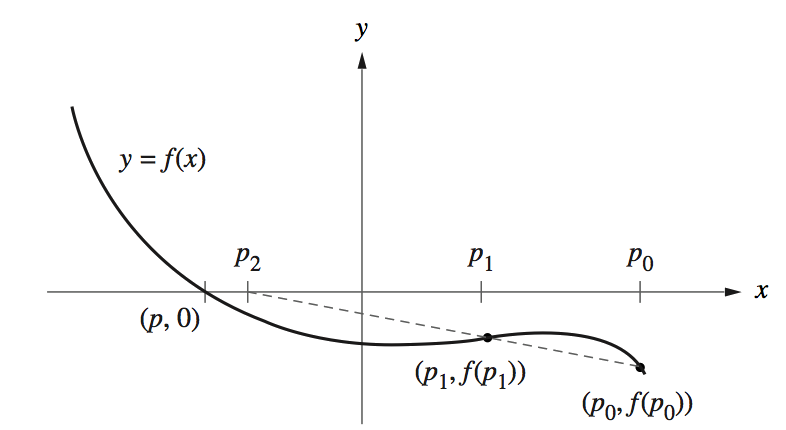
\includegraphics[width=45mm]{chap-1/fig_2-16.png}
\caption{The geometric construction of $p_2$ for the secant method.}
\end{center}
\end{figure}
}

\frame{
The values of $m$ in above equation are the slope of the secant line through the first two approximations and the slope of the line through $(p_1, f (p_1))$ and $(p_2, 0)$, respectively.
\begin{center}
$\Downarrow $
\end{center}
solve for $p_2 = g(p_1, p_0)$ and get
\begin{equation*}
p_2 = g(p_1,p_0)  = p_1 - {f(p_1)(p_1-p_0)}{f(p_1)-f(p_0)}
\end{equation*}
\begin{center}
$\Downarrow $
\end{center}
The general term is given by the two-point iteration formula
\begin{equation*}
p_{k+1} = g(p_k,p_{k-1})  = p_k - {f(p_k)(p_k-p_{k-1})}{f(p_k)-f(p_{k-1})}
\end{equation*}
}

\frame{
\frametitle{Accelerated Convergence}
\begin{itemize}
\item We could hope that there are root-finding techniques that converge faster than linearly when $p$ is a root of order $M$. 
\item Our final result shows that a modification can be made to Newton’s method so that convergence becomes quadratic at a multiple root.
\end{itemize}
}

\frame{
\begin{block}{Theorem  (Acceleration of Newton-Raphson Iteration).}
Suppose that the Newton-Raphson algorithm produces a sequence that converges linearly to the root $x = p$ of order $M > 1$. 
Then the Newton-Raphson iteration formula
\begin{equation*}
p_k = p_{k-1} - \frac{M f(p_{k-1})}{f'(p_{k-1})}
\end{equation*}
will produce a sequence $\{ p_k \}^{\infty}_{k = 0}$ that converges quadratically to $p$.
\end{block}
}


